\section{Threat Model and Objectives}
\label{sec:threat}

\begin{figure}[t]
\centering
\IfFileExists{figures/fig_observation.pdf}{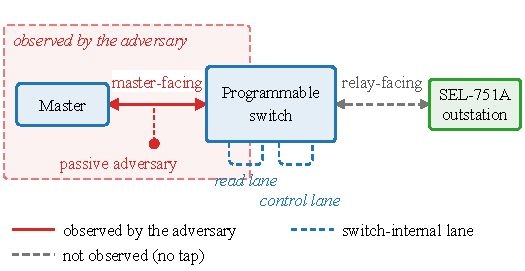
\includegraphics{figures/fig_observation}}{\figplaceholder{Topology and observation model. Master $\rightarrow$ observed master-facing link $\rightarrow$ programmable switch at the outstation edge $\rightarrow$ SEL-751 relay. The passive adversary sees only the master-facing link (solid); the relay-facing link and the two switch-internal scheduling lanes (dashed) are not observed.}}
\caption{Observation model. The master reaches the SEL-751 outstation through one programmable switch
at the outstation edge. The passive adversary observes only the master-facing link; the relay-facing
link and the switch-internal scheduling lanes are not observed.}
\label{fig:observation}
\end{figure}

\textbf{Assumptions on the adversary.} We adopt the threat model of Formby et
al.~\cite{formbyWhosControlYour2016}. Figure~\ref{fig:observation} shows the setup. The adversary is passive: it
observes the master-facing link,
records TCP and IP headers, segment sizes, and arrival times, and neither modifies nor injects a
packet. Because legacy DNP3 usually runs without transport security across shared substation
networks~\cite{eastTaxonomyAttacksDNP32009}, we assume the traffic is unencrypted. Consequently, the adversary reads the
exchange directly, and its advantage comes from observing it, not from a secret.

\textbf{Reconnaissance target.} The adversary fingerprints the outstation to prepare a later attack.
Because a control-related attack, such as a false-data injection attack, works only when the attacker
knows the target device~\cite{liuFalseDataInjection2009}, this reconnaissance is the enabling step. The fingerprint
survives without decoding the payload, because it is carried by the timing of the exchange. Following
Formby et al.~\cite{formbyWhosControlYour2016}, two timing features are in scope: the interval between the
transport-layer acknowledgment and the application-layer response on a read, i.e., the cross-layer
response time (CLRT); and the interval between a control request and its response, i.e., the operation
time. The first reflects the outstation's internal processing, and the second reveals the physical
device behind the control command.

\textbf{Objectives.} Our objective is to remove these two features from the master-facing observation.
We state it as three properties that anchor the design and the evaluation.
\begin{itemize}
  \item \textbf{RO1 (read timing).} The master-visible CLRT is a fixed policy value, independent of
    the transaction, so it no longer reflects the outstation's native processing.
  \item \textbf{RO2 (control timing).} The master-visible operation time is a fixed policy value,
    independent of the switch-internal release delay.
  \item \textbf{RO3 (safety).} The defense actuates no physical output.
\end{itemize}

\textbf{For active and relay-facing adversaries.} An adversary that manipulates traffic, breaks a
protected channel, or observes the relay-facing link is out of scope. Passive observation of the
master-facing link is the setting that prior traffic-obfuscation work targets and the one an
unencrypted deployment exposes; we leave the others to future work.

\textbf{For packet-size fingerprinting.} We do not obfuscate the outstation's response length. Our
scope is the two timing features above, and the response length is not a target of this defense.
